\documentclass{standalone}

\usepackage{tikz}
\usepackage{standalone}
\usetikzlibrary{calc}

\begin{document}
    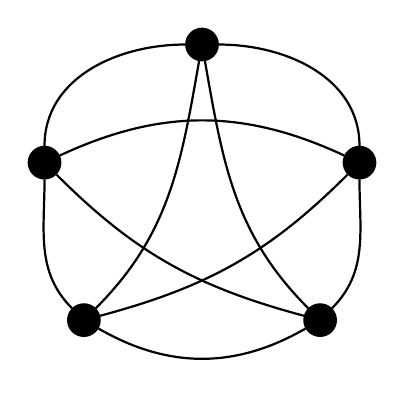
\begin{tikzpicture}

    \tikzstyle{state}=[minimum width=0.4cm, font=\boldmath];


    \node[circle, draw, fill, thick] (0) at (0, 1.5) [state]   {};
    \node[circle, draw, fill, thick] (1) at (-2, 0) [state]  {};
    \node[circle, draw, fill, thick] (2) at (-1.5, -2) [state] {};
    \node[circle, draw, fill, thick] (3) at (1.5, -2) [state]  {};
    \node[circle, draw, fill, thick] (4) at (2, 0) [state]   {};

    \draw (0) edge[out=180, in=90, -, thick] node [above] {} (1);
    \draw (0) edge[out=0, in=90, -, thick] node [above] {} (4);
    \draw (1) edge[out=-90, in=135, -, thick] node [above] {} (2);
    \draw (2) edge[out=-30, in=-150, -, thick] node [above] {} (3);
    \draw (4) edge[out=-90, in=45, -, thick] node [above] {} (3);

    \draw (2) edge[out=15, in=-135, -, thick] node [above] {} (4);
    \draw (3) edge[out=165, in=-45, -, thick] node [above] {} (1);

    \draw (0) edge[out=-100, in=45, -, thick] node [above] {} (2);
    \draw (0) edge[out=-80, in=135, -, thick] node [above] {} (3);

    \draw (1) edge[out=25, in=155, -, thick] node [above] {} (4);
    \end{tikzpicture}
\end{document}